\documentclass[final]{beamer}
% http://tex.stackexchange.com/questions/56205/wrapfigure-beamer-style
\usepackage{color}
\usepackage{transparent}
%\usepackage{enumitem}
%\usepackage{cutwin}
%\usetheme{RJH}
\usetheme{Berkeley}
%\usetheme{Bergen}
\usepackage[orientation=portrait,size=a0,scale=1.4,debug]{beamerposter}
\usepackage[absolute,overlay]{textpos}
\setlength{\TPHorizModule}{1cm}
\setlength{\TPVertModule}{1cm}
\beamertemplatenavigationsymbolsempty
% RGB (145,201,219), #91C9DB
%\definecolor{mybluelabel}{RGB}{145,201,219}
% RGB (48,174,228), #30AEE4
\definecolor{mybluelabel}{RGB}{48,174,228}

% Turn off list indentation
%\setlist[itemize]{leftmargin=*}

\begin{document}
\begin{frame}{} 

%\begin{textblock}{20}(2,2)
%\begin{center}
%\begin{figure}[tbph]
%\centering
%%\includegraphics[width=0.45\textwidth]{dianahep-logo.png}
%
\includegraphics[width=0.70\textwidth]{images/diana-hep-06-logo-horizontal.png}
%\end{figure}
%\url{http://s2i2-hep.org}
%\end{center}
%\end{textblock}



\begin{textblock}{84.0}(1,2)
\begin{center}
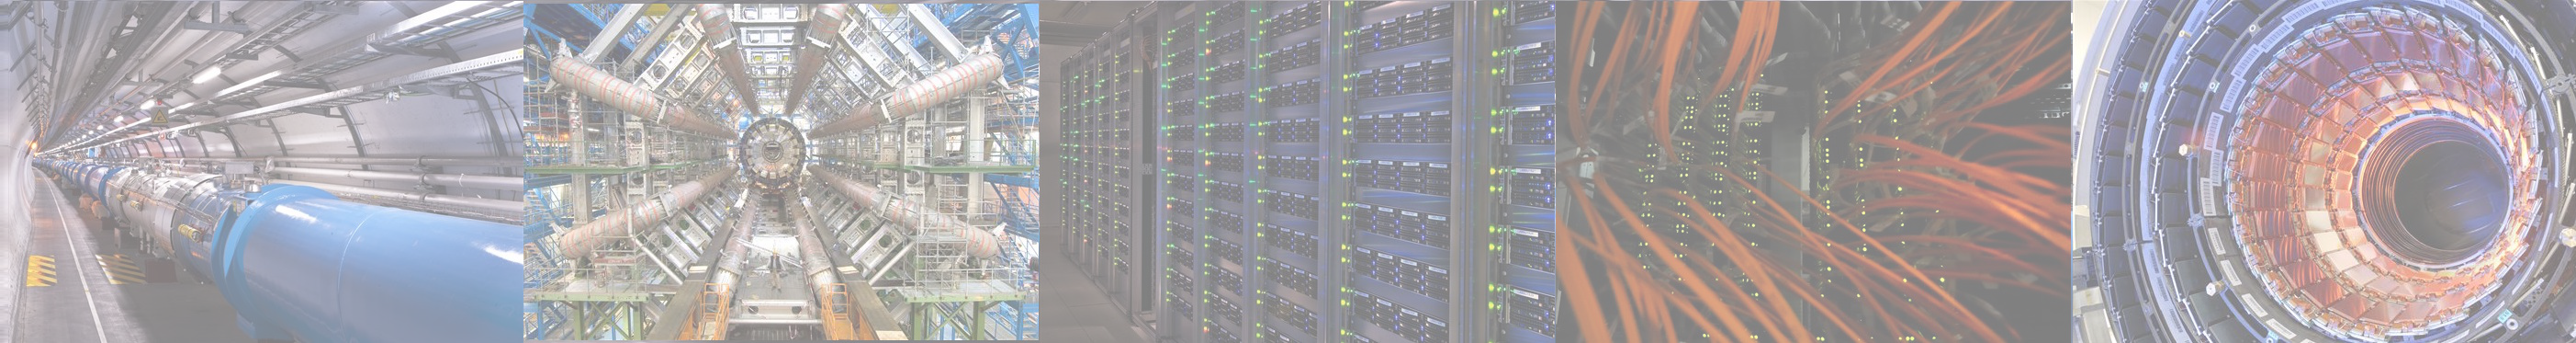
\includegraphics[width=0.95\textwidth]{images/s2i2-banner-50percent.png}
\end{center}
\end{textblock}

\begin{textblock}{84.0}(1,3)
\begin{center}
\begin{Huge}
%\color{white}{
\textbf{
Conceptualization of an S2I2 Institute \\
~~for High Energy Physics (S2I2-HEP)
}
%}
\end{Huge}
\end{center}
\end{textblock}

\begin{textblock}{84.0}(2,8.8)
\begin{center}
\begin{Large}
\textbf{
PIs: Peter Elmer (Princeton Univ.), Mark Neubauer (Univ. of Illinois \\ 
at Urbana-Champaign), Mike Sokoloff (Univ. of Cincinnati)
}
\end{Large}
\end{center}
\end{textblock}

\begin{textblock}{78.0}(4,14)
\begin{block}{The S2I2-HEP Project}
The primary goal of the S2I2-HEP conceptualization project is to
prepare a strategic plan for a potential NSF Scientific Software
Innovation Institute (S2I2) to develop software for experiments
taking data in the ``High-Luminosity Large Hadron Collider'' (HL-LHC)
era in the 2020s. In addition, we are working with the HEP Software
Foundation to prepare a larger HEP Community White Paper (CWP)
with a global roadmap for HEP Software and Computing R\&D for
the 2020s. 
This project is supported by National Science Foundation grants ACI-1558216, ACI-1558219, and ACI-1558233. Any opinions, findings, conclusions or recommendations expressed in this material are those of the developers and do not necessarily reflect the views of the National Science Foundation.

\end{block}
\end{textblock}

\begin{textblock}{38.0}(4,25)
\begin{block}{High Energy Physics (HEP)}
%\begin{center}
The quest to understand the fundamental building blocks of nature,
and their interactions, is one of the longest running and most
ambitious of human endeavors. Facilities such as the Large Hadron
Collider (LHC), where we do our research, represent a huge step
forward in our ability to answer these questions. The discovery of
the Higgs boson, the observation of exceedingly rare decays of B
mesons, and exclusion of countless theories beyond the Standard
Model (SM) of particle physics demonstrate that these experiments
deliver results. However, the most interesting fundamental physics
questions remain wide open, amongst them: What is the dark matter
which pervades the universe? Does space-time have additional
symmetries or extend beyond the 3 spatial dimensions we know? What
is the mechanism stabilizing the Higgs mass from enormous quantum
corrections? Are neutrinos, whose only SM interactions are weak,
their own anti-particles? Can the theories of gravity and quantum
mechanics be reconciled? Planned and running HEP experiments 
and facilities aim to answer these questions over the next 20 years. 
The computing and software challenges of these projects are formidable. 
The LHC experiments, for example, use nearly 0.5 Exabyte of
storage today in 170 computer centers in 42 countries. 
The upgrade to the High-Luminosity Large Hadron Collider (HL-LHC) will
increase the data volume
by more than a factor of 100, with significantly increased data and detector complexity. The resulting computing needs will outpace the expected improvements in computer performance (Moore's Law) by factors of between 3 and 30. 

\begin{figure}[tbph]
\centering
%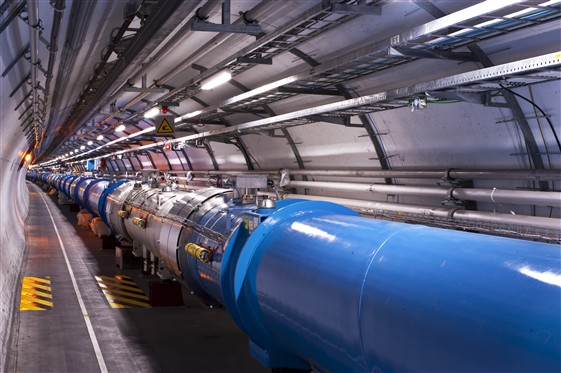
\includegraphics[width=0.48\textwidth]{images/0910152_02-A5-at-72-dpi.jpg}
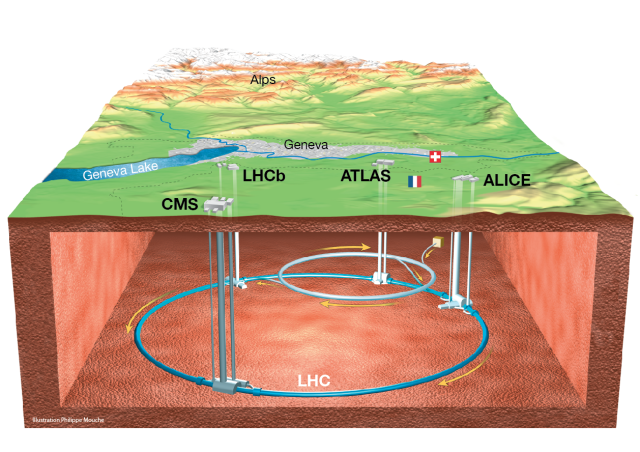
\includegraphics[width=0.41\textwidth]{images/CERN-LHC-cutaway-view-medium.png}
%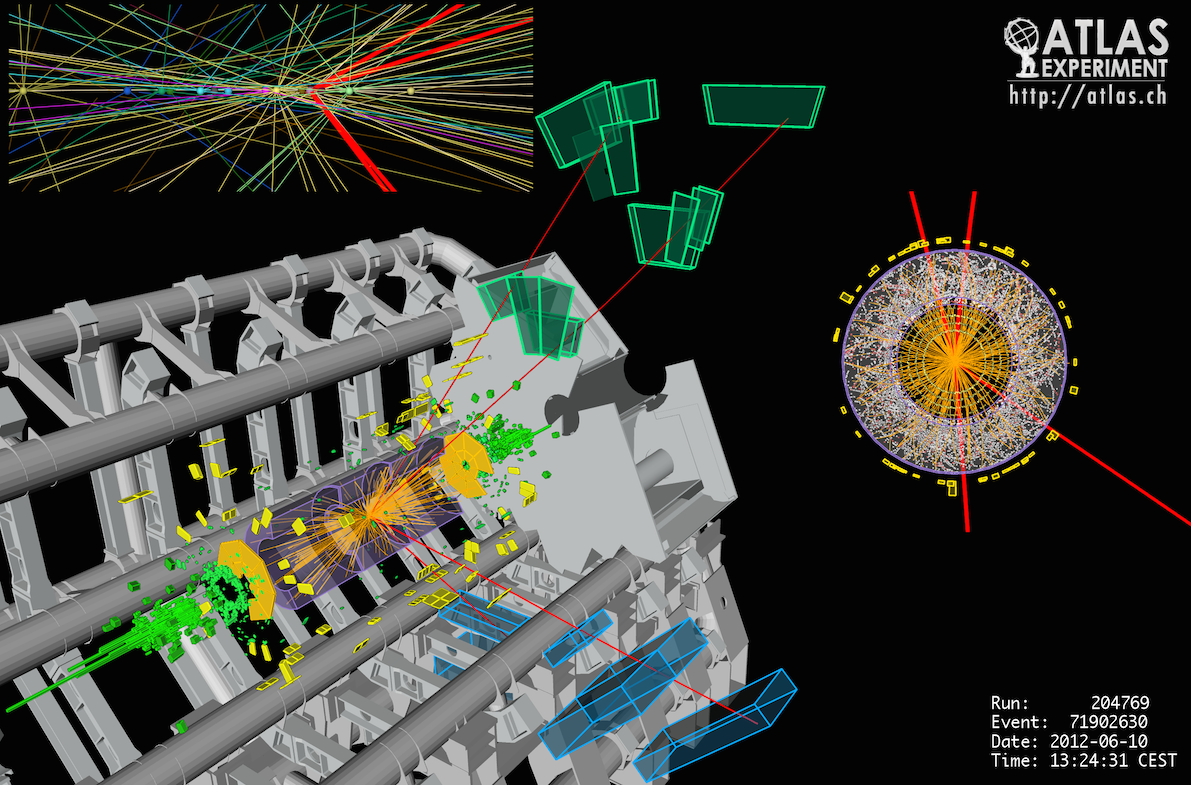
\includegraphics[width=0.41\textwidth]{images/run204769_evt71902630_VP1Base-half.png}
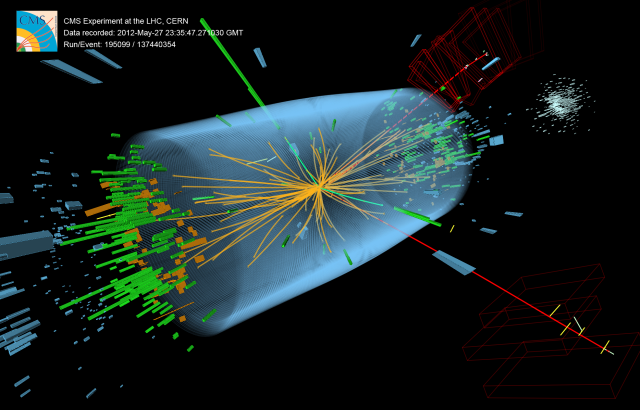
\includegraphics[width=0.42\textwidth]{images/eemm_run195099_evt137440354_ispy_3d-annotated-2.png}
%\begin{center}
%\end{center}
\end{figure}
{\small \copyright~2009-2016 CERN (License: CC-BY-SA-4.0)}
\end{block}
\end{textblock}

%\begin{textblock}{38.0}(4,65)
%\begin{block}{High-Luminosity Large Hadron Collider (HL-LHC)}
%\end{block}
%\end{textblock}


\begin{textblock}{38.0}(4,75)
\begin{block}{HSF Community White Paper Workshop at SDSC, 23-26 Jan 2017}
This was the first CWP workshop, organized jointly by S2I2-HEP and the HEP Software Foundation (\url{http://hepsoftwarefoundation.org}). The aim of this workshop was to begin the CWP process, formulate charges and plans for the CWP working groups. It consisted of plenary sessions, parallels and topical panels with 120 attendees from HEP, Computer Science and Industry.
\begin{figure}[tbph]
\centering
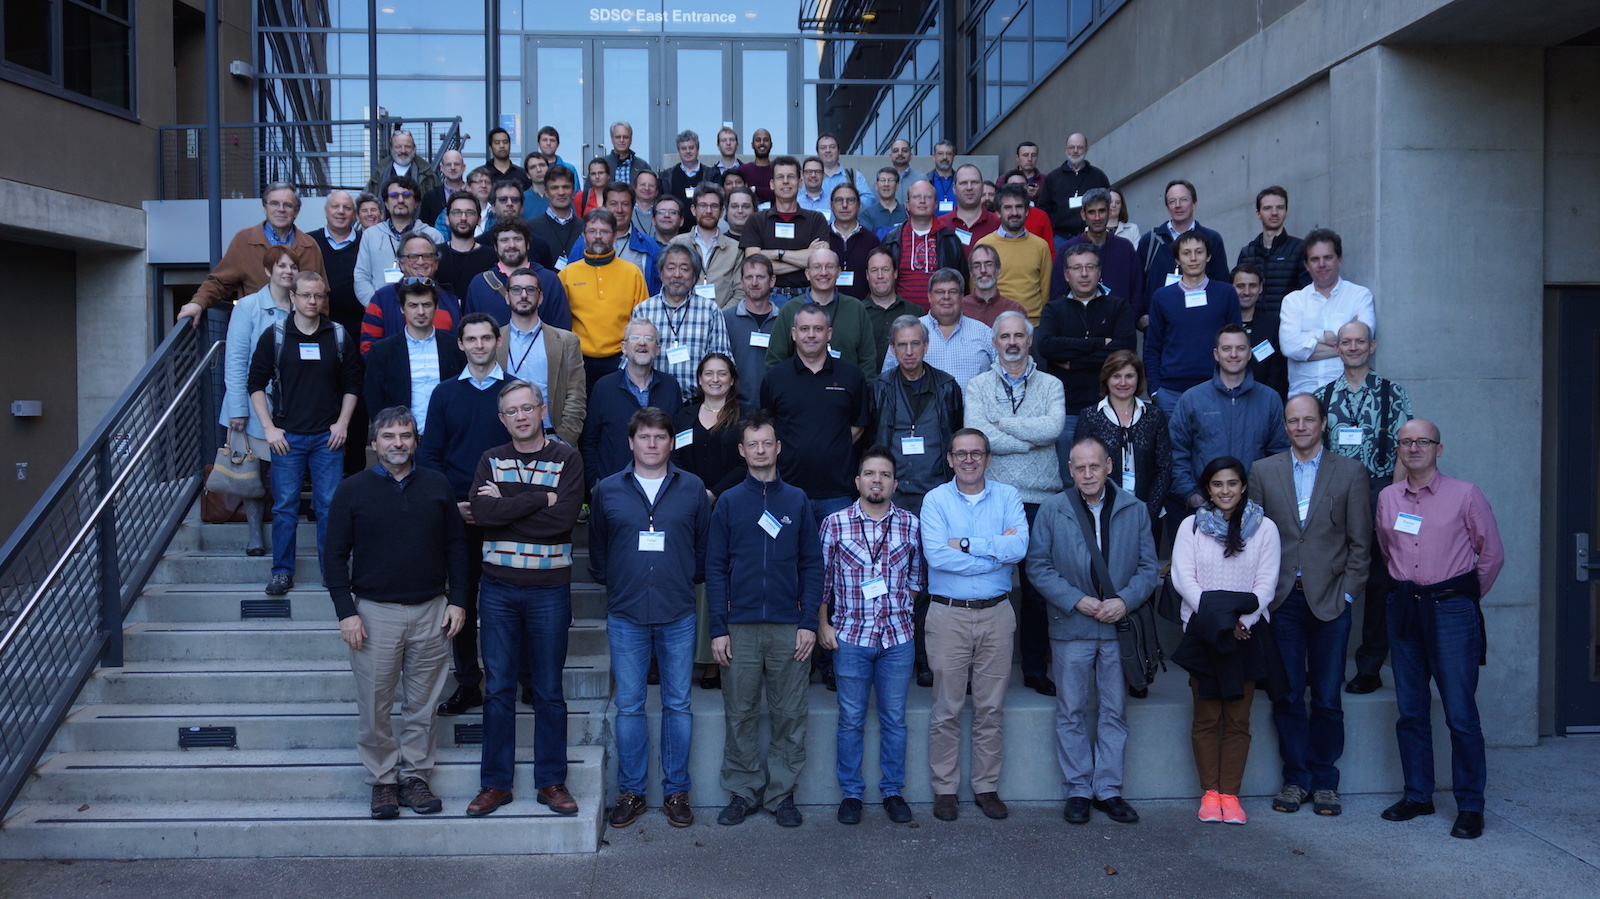
\includegraphics[width=0.50\textwidth]{images/20170125-HSF-SDSC-Workshop-group-photo.jpg}
\end{figure}
Topics covered included simulation, data analysis and interpretation, event processing frameworks, workflow and resource management, triggering and reconstruction, data analytics and machine learning, data access and management, visualization, data and software preservation and software development, deployment and validation. \\
{\small Meeting agenda: \url{http://indico.cern.ch/event/570249/}} \\



\begin{textblock}{38.0}(44,82.5)
\begin{block}{Future S2I2-HEP and HSF/CWP activities}
Outreach/sessions will be taking place during the collaboration meetings
of the large LHC and HEP experiments, as well as at large labs. We are also 
planning several additional S2I2 and/or CWP workshops before 
Summer 2017: \\
\begin{itemize}
\item 9 Mar, 2017 - Software Triggers and Event Reconstruction WG meeting
    \begin{itemize}
    \item LAL (Orsay), session at the Connecting The Dots workshop 
    \end{itemize}
\item 20-22 Mar, 2017 - IML Topical Machine Learning Workshop
    \begin{itemize}
    \item CERN, will include a CWP session on Machine Learning
    \end{itemize}
\item Early May, 2017 - Second S2I2 HEP/CS workshop
    \begin{itemize}
    \item Princeton (TBC)
    \end{itemize}
\item 22-24 May, 2017 - HEP Analysis Ecosystem Retreat
    \begin{itemize}
    \item Location TBD
    \end{itemize}
\item 5-6 Jun, 2017 - CWP Event Processing Frameworks Workshop (TBC)
    \begin{itemize}
    \item FNAL, just prior to the FNAL 50th Anniversary and User Meeting
    \end{itemize}
\item 26-30 Jun, 2017 - HEP Software Foundation Workshop
    \begin{itemize}
    \item LAPP (Annecy), Final CWP workshop
    \end{itemize}
\end{itemize}
In addition we are investigating the possibility of an S2I2-HEP ``writing'' meeting at the ACAT 2017 conference in Seattle the week of 21-25 Aug, 2017.
~~~ \\
The plan is to deliver the HSF Community White Paper document by the end of summer, 2017, and a final NSF S2I2-HEP strategic plan by the end of 2017.
\end{block}
\end{textblock}



\begin{textblock}{38.0}(44,25)
\begin{block}{S2I2-HEP and the HEP Software Foundation}
Our S2I2-HEP strategic plan will describe how an NSF S2I2, and the
U.S.\ university community, could provide leadership and enable the
science of the HL-LHC era.  HEP experiments involve international
collaborations and a global software ecosystem, however, and the
activities of a possible S2I2 for HEP would need to fit into a
larger international context. To that end, we are also working with
the HEP Software Foundation (HSF) to develop on the same time scale
a ``Community White Paper'' (CWP) with a global roadmap for HEP
Software and Computing R\&D for the 2020s. The aim of the CWP is
to identify and prioritise the software research and development
investments required:

\begin{itemize}
\item to achieve improvements in software efficiency, scalability and performance and to make use of the advances in CPU, storage and network technologies
\item to enable new approaches to computing and software that could radically extend the physics reach of the detectors
\item to ensure the long term sustainability of the software through the lifetime of the HL-LHC
\end{itemize}

Achieving consensus in a large international community is a complex task. We are modeling the CWP process on that used for the HEP ``decadal survey'' (Snowmass) process and using a mix of dedicated general and topical workshops, solicitations for topical white papers contributions and outreach sessions at pre-existing HEP meetings. Most major HEP stakeholders (experiments, labs, institutions, software projects) are being engaged.
\end{block}
\end{textblock}




\begin{textblock}{38.0}(44,63)
\begin{block}{S2I2 HEP/CS workshop at NCSA, 7-9 Dec 2016}
The first S2I2-HEP workshop focused on fostering collaboration between the HEP and Computer Science communities. There were 50 attendees, with about half from HEP and half from Computer Science.
\begin{figure}[tbph]
\centering
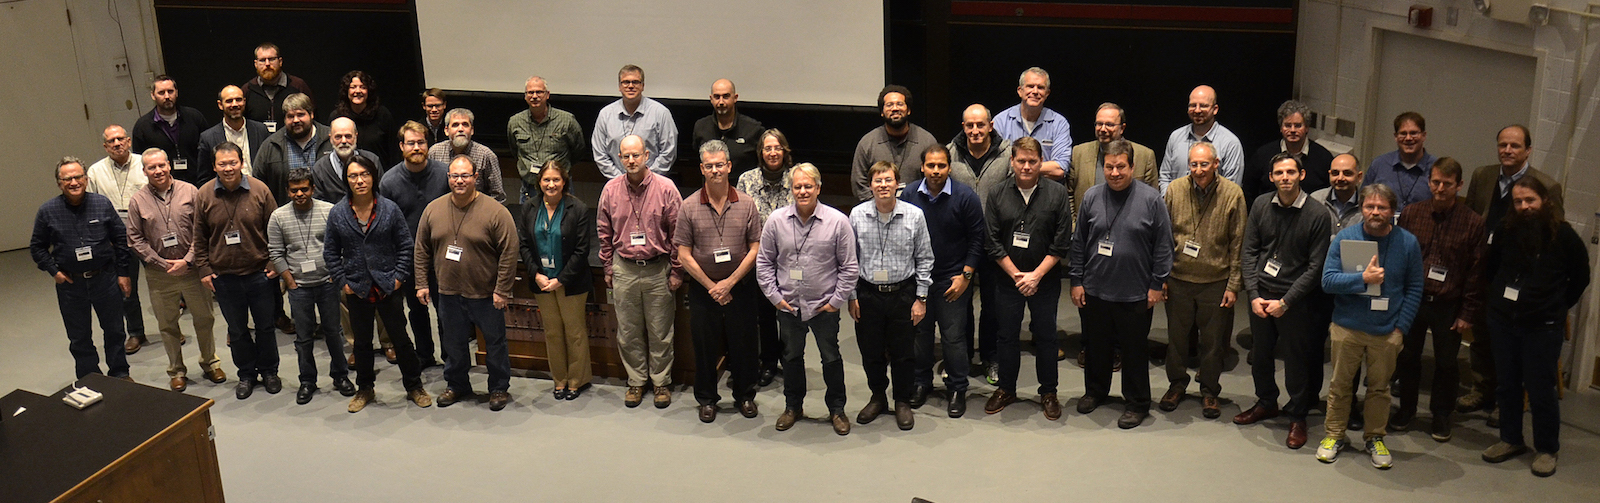
\includegraphics[width=0.60\textwidth]{images/20161208-s2i2-hep-cs-group-photo.jpg}
\end{figure}
{\small Meeting agenda: \url{https://indico.cern.ch/event/575443/}} \\
{\small Summary: \url{http://s2i2-hep.org/downloads/s2i2-hep-cs-workshop-summary.pdf}}
\end{block}
\end{textblock}

\end{block}
\end{textblock}




\begin{textblock}{14.0}(4,107)
\begin{block}{This poster online with links}
\begin{figure}[tbph]
\centering

\includegraphics[width=0.30\textwidth]{images/qr-s2i2-hep-si2-pi-workshop-2017.png}
\end{figure}
\begin{center}
\url{http://goo.gl/k22mD9}
\end{center}
\end{block}
\end{textblock}


\begin{textblock}{14.0}(20,107)
\begin{block}{S2I2-HEP Project website}
\begin{figure}[tbph]
\centering

\includegraphics[width=0.30\textwidth]{images/qr-s2i2-hep.png}
\end{figure}
\begin{center}
\url{http://s2i2-hep.org}
\end{center}
\end{block}
\end{textblock}

\begin{textblock}{10.0}(34,107)
%\begin{block}{This poster online with links}
\begin{figure}[tbph]
\centering

\includegraphics[width=0.75\textwidth]{images/nsf1.jpg}
\end{figure}
%\end{block}
\end{textblock}


%\begin{textblock}{38.0}(44,109)
%\begin{block}{Acknowledgement}
%\end{block}
%\end{textblock}




\end{frame}
\end{document}
